\documentclass[11pt,a4paper]{article}

% Packages
\usepackage[margin=2.3cm]{geometry}
\usepackage[protrusion=true,expansion=false]{microtype}
\usepackage{graphicx}
\usepackage{tikz}
\usetikzlibrary{shapes,arrows.meta,positioning,calc,fit,backgrounds,shadows.blur,decorations.pathmorphing,decorations.pathreplacing}
\usepackage{colortbl}
\usepackage{enumitem}
\usepackage{booktabs}
\usepackage{longtable}
\usepackage{array}
\usepackage{hyperref}
\usepackage{xcolor}
\usepackage{fancyhdr}
\usepackage{titlesec}
\usepackage[most]{tcolorbox}
\usepackage{amsmath,amssymb}
\usepackage{setspace}
\usepackage{fontawesome5}
\usepackage{listings}

% Spacing
\setlength{\parskip}{3pt plus 1pt minus 1pt}
\setlength{\parindent}{0pt}
\renewcommand{\arraystretch}{1.25}

% Colors
\definecolor{primary}{HTML}{1A5276}
\definecolor{secondary}{HTML}{2E86C1}
\definecolor{accent}{HTML}{E74C3C}
\definecolor{lightbg}{HTML}{EBF5FB}
\definecolor{defbg}{HTML}{FDF2E9}
\definecolor{greenhl}{HTML}{27AE60}
\definecolor{purplehl}{HTML}{8E44AD}
\definecolor{codebg}{HTML}{F4F6F7}

% Hyperref
\hypersetup{colorlinks=true, linkcolor=primary, urlcolor=secondary, citecolor=primary}

% Code listings style
\lstset{
  backgroundcolor=\color{codebg},
  basicstyle=\ttfamily\small,
  keywordstyle=\color{primary}\bfseries,
  stringstyle=\color{greenhl},
  commentstyle=\color{gray}\itshape,
  breaklines=true,
  frame=l,
  framerule=2pt,
  rulecolor=\color{secondary!40},
  xleftmargin=8pt,
  framexleftmargin=6pt,
  aboveskip=6pt,
  belowskip=6pt,
  showstringspaces=false,
  language=R
}

% Header/Footer
\pagestyle{fancy}
\fancyhf{}
\fancyhead[L]{\small\textcolor{primary}{\textbf{Data Science --- Final Solution Key}}}
\fancyhead[R]{\small\textcolor{primary}{BSIT}}
\fancyfoot[C]{\small\thepage}
\renewcommand{\headrulewidth}{0.5pt}
\renewcommand{\footrulewidth}{0.3pt}

% Section formatting
\titleformat{\section}{\large\bfseries\color{primary}}{}{0em}{}[\vspace{2pt}\titlerule]
\titlespacing*{\section}{0pt}{14pt}{8pt}

% Custom boxes
\newtcolorbox{definitionbox}[1][]{
  enhanced, breakable,
  colback=defbg, colframe=orange!60!black,
  colbacktitle=orange!70!black, coltitle=white,
  title={\faIcon{book}~#1}, fonttitle=\bfseries,
  boxrule=0pt, leftrule=4pt, arc=2pt,
  shadow={1mm}{-1mm}{0mm}{black!15},
  top=4pt, bottom=4pt, left=8pt, right=8pt
}
\newtcolorbox{conceptbox}[1][]{
  enhanced, breakable,
  colback=lightbg, colframe=secondary,
  colbacktitle=secondary, coltitle=white,
  title={\faIcon{lightbulb}~#1}, fonttitle=\bfseries,
  boxrule=0pt, leftrule=4pt, arc=2pt,
  shadow={1mm}{-1mm}{0mm}{black!15},
  top=4pt, bottom=4pt, left=8pt, right=8pt
}
\newtcolorbox{warnbox}[1][]{
  enhanced, breakable,
  colback=accent!8, colframe=accent,
  colbacktitle=accent, coltitle=white,
  title={\faIcon{exclamation-triangle}~#1}, fonttitle=\bfseries,
  boxrule=0pt, leftrule=4pt, arc=2pt,
  shadow={1mm}{-1mm}{0mm}{black!15},
  top=4pt, bottom=4pt, left=8pt, right=8pt
}

% Question header box
\newtcolorbox{qbox}[1][]{
  enhanced, breakable,
  colback=primary!8, colframe=primary,
  boxrule=0pt, leftrule=4pt, arc=2pt,
  top=4pt, bottom=4pt, left=8pt, right=8pt,
  fontupper=\bfseries
}

\newcommand{\question}[3][05 marks]{%
  \begin{qbox}#2\hfill\textcolor{accent}{(#1)}\\[2pt]#3\end{qbox}%
}

\begin{document}

% Title
\begin{center}
\vspace*{0.3cm}
{\Huge\bfseries\textcolor{primary}{Final Exam --- Solution Key}}\\[8pt]
{\Large\bfseries\textcolor{primary}{Data Science, AI \& Emerging Paradigms}}\\[14pt]
{\color{secondary}\rule{0.6\textwidth}{1.5pt}}\\[12pt]
{\Large\textsc{BSIT --- Data Science}}\\[6pt]
{\large\textcolor{gray!70!black}{Worked, To-the-Point Answers Grounded in the Course Handouts}}
\vspace{0.2cm}
\end{center}

%=============================================================
\question[02 marks]{Q-1. Differentiate between the three levels of analytics: Descriptive, Predictive, and Prescriptive.}{}

The three levels form a \textbf{maturity ladder}: each level answers a harder question and delivers more decision value than the one before it.

\begin{center}
\begin{tabular}{@{}>{\bfseries}p{2.6cm}p{3.4cm}p{4.0cm}p{4.0cm}@{}}
\toprule
\rowcolor{primary!15}
\textbf{Aspect} & \textbf{Descriptive} & \textbf{Predictive} & \textbf{Prescriptive} \\
\midrule
Question answered & What \emph{happened}? & What is \emph{likely} to happen? & What should we \emph{do} about it? \\
Focus & Past \& present data & Future outcomes & Best action / decision \\
Typical methods & Aggregation, summary statistics, dashboards, reports & Regression, classification, forecasting, ML models & Optimization, simulation, recommendation, decision rules \\
Output & Insight / description & Forecast / probability & Actionable recommendation \\
Example & ``Sales fell 12\% last quarter.'' & ``Sales will fall a further 8\% next quarter.'' & ``Cut price 5\% \& boost ad spend to recover sales.'' \\
\bottomrule
\end{tabular}
\end{center}

\begin{conceptbox}[Key Idea]
Complexity and business value \textbf{increase} from Descriptive $\rightarrow$ Predictive $\rightarrow$ Prescriptive. Descriptive looks \emph{backward}, Predictive looks \emph{forward}, and Prescriptive tells you \emph{what to do} --- often using the output of the predictive stage as its input.
\end{conceptbox}

%=============================================================
\question[02 marks]{Q-2. Explain the conceptual differences among Data Mining, Machine Learning, Deep Learning, and Data Science.}{}

These terms are related but sit at different \textbf{levels of scope}. Data Science is the broad umbrella; the others are nested capabilities used inside it.

\begin{center}
\begin{tabular}{@{}>{\bfseries}p{2.7cm}p{4.2cm}p{5.6cm}@{}}
\toprule
\rowcolor{primary!15}
\textbf{Term} & \textbf{What It Is} & \textbf{Core Focus} \\
\midrule
Data Science & The broad, multidisciplinary field of extracting knowledge from data & End-to-end lifecycle: collect, clean, analyse, model, visualise, communicate (stats + coding + domain) \\
Data Mining & The \emph{process} of discovering patterns / relationships in large datasets & Finding hidden patterns, associations, clusters, and anomalies \\
Machine Learning & A subset of AI: algorithms that \emph{learn} from data & Building models that predict or classify without being explicitly programmed \\
Deep Learning & A subset of ML using multi-layer neural networks & Learning complex patterns \& features automatically from images, text, audio \\
\bottomrule
\end{tabular}
\end{center}

\begin{center}
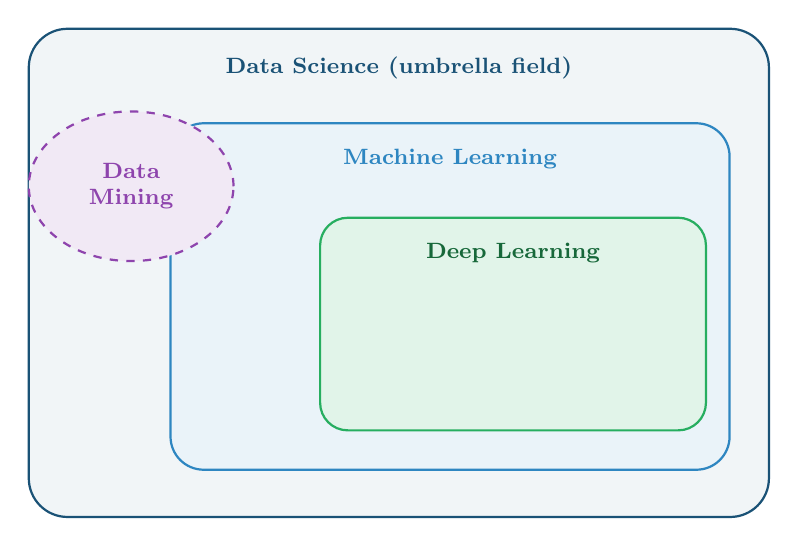
\begin{tikzpicture}[font=\footnotesize\bfseries]
  % Concentric containment: DS > ML > DL
  \draw[thick, primary, fill=primary!6, rounded corners=14pt] (-4.7,-3.1) rectangle (4.7,3.1);
  \node[primary] at (0,2.6) {Data Science (umbrella field)};

  \draw[thick, secondary, fill=secondary!10, rounded corners=12pt] (-2.9,-2.5) rectangle (4.2,1.9);
  \node[secondary] at (0.65,1.45) {Machine Learning};

  \draw[thick, greenhl, fill=greenhl!14, rounded corners=10pt] (-1.0,-2.0) rectangle (3.9,0.7);
  \node[greenhl!60!black] at (1.45,0.25) {Deep Learning};

  % Data Mining: overlapping set on the left
  \draw[thick, dashed, purplehl, fill=purplehl!12] (-3.4,1.1) ellipse (1.3cm and 0.95cm);
  \node[purplehl, align=center] at (-3.4,1.1) {Data\\Mining};
\end{tikzpicture}
\end{center}

\begin{conceptbox}[One-Line Summary]
\textbf{Deep Learning} $\subset$ \textbf{Machine Learning} $\subset$ tools used within \textbf{Data Science}; \textbf{Data Mining} is the pattern-discovery \emph{process} that overlaps both statistics and ML inside the Data Science workflow.
\end{conceptbox}

%=============================================================
\question[02 marks]{Q-3. Classify each customer variable as Numerical (Continuous / Discrete) or Categorical (Nominal / Ordinal / Binary).}{}

\begin{center}
\begin{tabular}{@{}>{\bfseries}p{3.6cm}p{3.4cm}p{6.0cm}@{}}
\toprule
\rowcolor{primary!15}
\textbf{Variable} & \textbf{Classification} & \textbf{Reason} \\
\midrule
Customer ID & Categorical --- Nominal & Just a label / identifier; the digits carry no magnitude or order (no averaging). \\
Name & Categorical --- Nominal & Text label with no inherent order. \\
Age & Numerical --- Discrete & Counted in whole years (integers). \emph{(Continuous if measured exactly.)} \\
Annual Income (\$) & Numerical --- Continuous & Can take any value on a scale, including decimals. \\
Satisfaction Level & Categorical --- Ordinal & Ordered categories: Low $<$ Medium $<$ High, but no fixed numeric gap. \\
Is-Active-Member & Categorical --- Binary & Exactly two categories (Yes / No). \\
Last Purchase Date & Temporal (Interval / Ordinal) & A date: values have a meaningful order and differences (days between), but no true zero. \\
\bottomrule
\end{tabular}
\end{center}

\begin{conceptbox}[Watch-Out]
A variable stored as \emph{numbers} is not automatically numerical. \textbf{Customer ID} looks numeric but is nominal, because arithmetic on it is meaningless. Always ask ``do order and arithmetic make sense?'' before choosing the type.
\end{conceptbox}

%=============================================================
\question[06 marks]{Q-4. Compare Single-Agent and Multi-Agent systems. When is multi-agent preferred? Give two advantages, two risks, and a concrete scenario.}{}

\begin{center}
\begin{tabular}{@{}>{\bfseries}p{2.6cm}p{5.3cm}p{5.3cm}@{}}
\toprule
\rowcolor{primary!15}
\textbf{Aspect} & \textbf{Single-Agent System} & \textbf{Multi-Agent System} \\
\midrule
Structure & One agent handles the whole task & Several specialized agents cooperate \\
Complexity & Simpler to build, monitor, and debug & More modular but more moving parts \\
Coordination & No inter-agent communication needed & Needs orchestration \& message passing \\
Best for & Focused, well-scoped tasks & Large workflows split into sub-tasks \\
\bottomrule
\end{tabular}
\end{center}

\textbf{When is a multi-agent architecture preferred?} When the problem can be \textbf{decomposed} into distinct sub-tasks that need different skills or tools, when sub-tasks can run \textbf{in parallel}, when the workflow is too large for one agent's context, or when \textbf{fault isolation} (one agent failing without taking down the rest) matters.

\vspace{2pt}
\begin{minipage}[t]{0.49\textwidth}
\begin{conceptbox}[Two Advantages]
\begin{itemize}[leftmargin=*,topsep=1pt,itemsep=2pt]
  \item \textbf{Specialization \& modularity:} each agent is an expert at one job, so it can be improved or replaced independently.
  \item \textbf{Parallelism \& scalability:} sub-tasks run at the same time, handling larger workloads faster.
\end{itemize}
\end{conceptbox}
\end{minipage}\hfill
\begin{minipage}[t]{0.49\textwidth}
\begin{warnbox}[Two Risks]
\begin{itemize}[leftmargin=*,topsep=1pt,itemsep=2pt]
  \item \textbf{Coordination overhead:} more communication means more latency, cost, and points of failure.
  \item \textbf{Error propagation \& unpredictability:} one agent's mistake can cascade, and emergent behaviour is harder to monitor and control.
\end{itemize}
\end{warnbox}
\end{minipage}

\begin{definitionbox}[Concrete Scenario --- an AI Grading \& Feedback System for a University]
\textbf{Single-agent design:} one agent reads each student's essay, grades it, and writes feedback. Simple, but it does everything sequentially and struggles when the workload (hundreds of scripts) or the rubric grows.

\smallskip
\textbf{Multi-agent design:} an \emph{Orchestrator} splits the work among a \emph{Retrieval agent} (pulls the rubric \& reference answers), a \emph{Grading agent} (scores against the rubric), a \emph{Feedback agent} (writes personalised comments), and a \emph{Plagiarism-check agent}.

\smallskip
\textbf{Advantages realised:} the grading and plagiarism agents run in \emph{parallel} across many scripts (scalability), and the rubric logic can be upgraded without touching the feedback writer (specialization).\\
\textbf{Risks realised:} if the Retrieval agent fetches the \emph{wrong} rubric, every downstream grade is wrong (error propagation), and coordinating four agents adds cost and makes a bad grade harder to trace --- so \textbf{guardrails, logging, and a human-in-the-loop review} are required.
\end{definitionbox}

%=============================================================
\question[06 marks]{Q-5. For the store dataset ($N=8$), compute Support, Confidence, Lift, and Conviction for \{Laptop, Mouse\} $\rightarrow$ \{Keyboard\}. Why can Confidence mislead, and what does Lift indicate?}{}

\textbf{Step 0 --- The 8 transactions.} ($\checkmark$ = item present in the basket)

\begin{center}
\begin{tabular}{@{}c ccc @{}}
\toprule
\rowcolor{primary!15}
\textbf{Txn} & \textbf{Laptop} & \textbf{Mouse} & \textbf{Keyboard} \\
\midrule
T1 & $\checkmark$ & $\checkmark$ & $\checkmark$ \\
T2 & $\checkmark$ & $\checkmark$ & $\checkmark$ \\
T3 & $\checkmark$ & $\checkmark$ & $\checkmark$ \\
T4 & $\checkmark$ & $\checkmark$ & $\checkmark$ \\
T5 & $\checkmark$ & $\checkmark$ & \\
T6 & $\checkmark$ &            & $\checkmark$ \\
T7 &            & $\checkmark$ & $\checkmark$ \\
T8 &            & $\checkmark$ & $\checkmark$ \\
\bottomrule
\end{tabular}
\end{center}

\textbf{Step 1 --- Count the baskets we need.}
\begin{itemize}[leftmargin=*,topsep=1pt]
  \item Contain \{Laptop, Mouse\} (antecedent $A$): T1--T5 $\Rightarrow$ \textbf{5}
  \item Contain \{Laptop, Mouse, Keyboard\} ($A \cup B$): T1--T4 $\Rightarrow$ \textbf{4}
  \item Contain \{Keyboard\} (consequent $B$): T1--T4, T6, T7, T8 $\Rightarrow$ \textbf{7}
\end{itemize}

\textbf{Step 2 --- Apply the formulas.}
\begin{align*}
\text{Support}(A\Rightarrow B) &= \frac{\text{count}(A\cup B)}{N} = \frac{4}{8} = \mathbf{0.50}\\[4pt]
\text{Confidence}(A\Rightarrow B) &= \frac{\text{Support}(A\cup B)}{\text{Support}(A)} = \frac{4/8}{5/8} = \frac{4}{5} = \mathbf{0.80}\\[4pt]
\text{Lift}(A\Rightarrow B) &= \frac{\text{Confidence}}{\text{Support}(B)} = \frac{0.80}{7/8} = \frac{0.80}{0.875} \approx \mathbf{0.914}\\[4pt]
\text{Conviction}(A\Rightarrow B) &= \frac{1-\text{Support}(B)}{1-\text{Confidence}} = \frac{1-0.875}{1-0.80} = \frac{0.125}{0.20} = \mathbf{0.625}
\end{align*}

\begin{center}
\begin{tabular}{@{}>{\bfseries}p{2.6cm}cp{7.6cm}@{}}
\toprule
\rowcolor{primary!15}
\textbf{Metric} & \textbf{Value} & \textbf{Interpretation} \\
\midrule
Support & 0.50 & The rule appears in half of all baskets --- fairly frequent. \\
Confidence & 0.80 & When Laptop \& Mouse are bought, Keyboard appears 80\% of the time. \\
Lift & 0.914 & $<1$: buying Laptop+Mouse makes Keyboard \emph{slightly less} likely than average --- a \textbf{negative} association. \\
Conviction & 0.625 & $<1$ confirms the rule is weaker than independence would predict. \\
\bottomrule
\end{tabular}
\end{center}

\begin{warnbox}[Why Confidence Alone Can Mislead]
Confidence is a high-looking \textbf{0.80}, yet Keyboard already appears in \textbf{7 of 8} baskets (Support$(B)=0.875$) on its own. So the ``80\%'' mostly reflects that keyboards are bought \emph{anyway}, not a real Laptop+Mouse effect. Confidence ignores the base rate of the consequent, so a common item will \emph{always} look strongly predicted.
\end{warnbox}

\begin{conceptbox}[What Lift Indicates]
Lift corrects for that base rate by comparing the rule to \textbf{random chance}:
\begin{itemize}[leftmargin=*,topsep=1pt]
  \item \textbf{Lift $>1$} $\rightarrow$ positive association (items bought together more than expected).
  \item \textbf{Lift $=1.0$} $\rightarrow$ \emph{independence}: the antecedent has \emph{no} effect on the consequent.
  \item \textbf{Lift $<1$} $\rightarrow$ negative association (as here: $0.914$ --- they slightly repel).
\end{itemize}
Here the impressive 0.80 confidence hides a lift below~1: the rule is actually \emph{not} useful.
\end{conceptbox}

%=============================================================
\question[06 marks]{Q-6. Explain the basic concepts of EDA using the \texttt{mtcars} dataset.}{}

\textbf{Exploratory Data Analysis (EDA)} is the first ``get-to-know-your-data'' stage: summarise structure, distributions, and relationships \emph{before} modelling. \texttt{mtcars} has \textbf{32 cars} (rows) and \textbf{11 variables} (\texttt{mpg}, \texttt{cyl}, \texttt{disp}, \texttt{hp}, \texttt{drat}, \texttt{wt}, \texttt{qsec}, \texttt{vs}, \texttt{am}, \texttt{gear}, \texttt{carb}).

\begin{enumerate}[leftmargin=*,topsep=2pt,itemsep=3pt]
  \item \textbf{Understand the structure.} Check dimensions and types first.
\begin{lstlisting}
dim(mtcars)   # 32 rows, 11 columns
str(mtcars)   # variable names and types
head(mtcars)  # first few rows
\end{lstlisting}

  \item \textbf{Summary statistics (central tendency \& spread).} Mean, median, quartiles, min/max.
\begin{lstlisting}
summary(mtcars)      # 5-number summary per column
mean(mtcars$mpg)     # ~ 20.09 miles/gallon
sd(mtcars$mpg)       # ~ 6.03 spread
\end{lstlisting}

  \item \textbf{Univariate analysis (one variable).} Look at each variable's distribution --- shape, skew, spread.
\begin{lstlisting}
hist(mtcars$mpg)     # distribution of fuel economy
boxplot(mtcars$hp)   # spread + outliers in horsepower
\end{lstlisting}

  \item \textbf{Categorical / discrete variables.} Use frequency tables for \texttt{cyl}, \texttt{am}, \texttt{gear}.
\begin{lstlisting}
table(mtcars$cyl)    # 4-cyl:11, 6-cyl:7, 8-cyl:14
table(mtcars$am)     # 0 = automatic, 1 = manual
\end{lstlisting}

  \item \textbf{Bivariate analysis (relationships).} A scatter plot reveals how two variables move together.
\begin{lstlisting}
plot(mtcars$wt, mtcars$mpg)  # heavier cars -> lower mpg
cor(mtcars$wt, mtcars$mpg)   # ~ -0.87 strong negative
\end{lstlisting}

  \item \textbf{Correlation matrix.} Rank which variables drive \texttt{mpg} most.
\begin{lstlisting}
cor(mtcars)   # mpg vs wt(-0.87), cyl(-0.85), disp, hp
\end{lstlisting}

  \item \textbf{Outliers \& missing values.} Boxplots flag outliers; \texttt{mtcars} has \textbf{no} missing values.
\begin{lstlisting}
sum(is.na(mtcars))   # 0 missing values
\end{lstlisting}
\end{enumerate}

\begin{conceptbox}[Key Insights from \texttt{mtcars} EDA]
Average fuel economy $\approx$ \textbf{20 mpg}; \texttt{mpg} is \textbf{strongly negatively} correlated with weight (\texttt{wt}), number of cylinders (\texttt{cyl}), and horsepower (\texttt{hp}) --- i.e.\ bigger, heavier, more powerful cars drink more fuel. EDA surfaces these patterns \emph{before} any model is trained.
\end{conceptbox}

%=============================================================
\question[06 marks]{Q-7. RMSE, MAE, and R$^2$: give the formula, plain-language meaning, and whether higher/lower is better. Why can RMSE and MAE rank two models differently?}{}

For $n$ observations with actual value $y_i$, prediction $\hat{y}_i$, and mean $\bar{y}$:

\begin{center}
\begin{tabular}{@{}>{\bfseries}p{1.7cm}p{4.6cm}p{5.4cm}c@{}}
\toprule
\rowcolor{primary!15}
\textbf{Metric} & \textbf{Formula} & \textbf{What It Measures (plain language)} & \textbf{Better} \\
\midrule
RMSE &
$\sqrt{\dfrac{1}{n}\displaystyle\sum_{i=1}^{n}(y_i-\hat{y}_i)^2}$ &
Typical prediction error in the \emph{same units} as the target; squaring makes it \textbf{penalise large errors} heavily. &
\textcolor{accent}{Lower} \\
\addlinespace
MAE &
$\dfrac{1}{n}\displaystyle\sum_{i=1}^{n}\lvert y_i-\hat{y}_i\rvert$ &
The \emph{average absolute} error; treats every error equally (linearly), so it is robust to outliers. &
\textcolor{accent}{Lower} \\
\addlinespace
R$^2$ &
$1-\dfrac{\sum (y_i-\hat{y}_i)^2}{\sum (y_i-\bar{y})^2}$ &
The \emph{proportion of variance} in the target explained by the model (1 = perfect, 0 = no better than the mean). &
\textcolor{greenhl}{Higher} \\
\bottomrule
\end{tabular}
\end{center}

\textbf{Why might RMSE and MAE rank two models differently?} Because \textbf{RMSE squares the errors} before averaging, it punishes a few \emph{large} errors far more than MAE does. So a model with one big miss can look worse on RMSE while looking better on MAE (and vice-versa). Note $\text{RMSE} \ge \text{MAE}$ always, and the gap grows with the \emph{variance} of the errors (i.e.\ with outliers).

\begin{definitionbox}[Worked Example --- the Ranking Flips]
Five predictions each; look at the absolute errors:

\smallskip
\textbf{Model A} errors $= \{0,0,0,0,5\}$ \quad(four perfect, one big miss)\\
\textbf{Model B} errors $= \{2,2,2,2,2\}$ \quad(consistently mediocre)

\smallskip
\begin{tabular}{@{}lcc@{}}
\toprule
\rowcolor{primary!15}
& \textbf{MAE} & \textbf{RMSE} \\
\midrule
Model A & $\tfrac{0+0+0+0+5}{5}=\mathbf{1.00}$ & $\sqrt{\tfrac{0+0+0+0+25}{5}}=\sqrt{5}\approx\mathbf{2.24}$ \\
Model B & $\tfrac{2+2+2+2+2}{5}=\mathbf{2.00}$ & $\sqrt{\tfrac{4+4+4+4+4}{5}}=\sqrt{4}=\mathbf{2.00}$ \\
\bottomrule
\end{tabular}

\smallskip
\textbf{MAE prefers Model A} (1.00 $<$ 2.00), but \textbf{RMSE prefers Model B} (2.00 $<$ 2.24). The single large error in Model~A is amplified by squaring, so the two metrics \emph{disagree} on which model is best.
\end{definitionbox}

\begin{conceptbox}[Which to Trust?]
If a few large errors are especially costly (e.g.\ badly under-stocking a hospital), prefer \textbf{RMSE}. If all errors matter equally and you want robustness to outliers, prefer \textbf{MAE}. Report \textbf{R$^2$} alongside either to show \emph{how much} of the variation the model actually explains.
\end{conceptbox}

\end{document}
